\documentclass[a4paper, 11pt]{article}\usepackage[]{graphicx}\usepackage[]{color}
%% maxwidth is the original width if it is less than linewidth
%% otherwise use linewidth (to make sure the graphics do not exceed the margin)
\makeatletter
\def\maxwidth{ %
  \ifdim\Gin@nat@width>\linewidth
    \linewidth
  \else
    \Gin@nat@width
  \fi
}
\makeatother

\definecolor{fgcolor}{rgb}{0.345, 0.345, 0.345}
\newcommand{\hlnum}[1]{\textcolor[rgb]{0.686,0.059,0.569}{#1}}%
\newcommand{\hlstr}[1]{\textcolor[rgb]{0.192,0.494,0.8}{#1}}%
\newcommand{\hlcom}[1]{\textcolor[rgb]{0.678,0.584,0.686}{\textit{#1}}}%
\newcommand{\hlopt}[1]{\textcolor[rgb]{0,0,0}{#1}}%
\newcommand{\hlstd}[1]{\textcolor[rgb]{0.345,0.345,0.345}{#1}}%
\newcommand{\hlkwa}[1]{\textcolor[rgb]{0.161,0.373,0.58}{\textbf{#1}}}%
\newcommand{\hlkwb}[1]{\textcolor[rgb]{0.69,0.353,0.396}{#1}}%
\newcommand{\hlkwc}[1]{\textcolor[rgb]{0.333,0.667,0.333}{#1}}%
\newcommand{\hlkwd}[1]{\textcolor[rgb]{0.737,0.353,0.396}{\textbf{#1}}}%
\let\hlipl\hlkwb

\usepackage{framed}
\makeatletter
\newenvironment{kframe}{%
 \def\at@end@of@kframe{}%
 \ifinner\ifhmode%
  \def\at@end@of@kframe{\end{minipage}}%
  \begin{minipage}{\columnwidth}%
 \fi\fi%
 \def\FrameCommand##1{\hskip\@totalleftmargin \hskip-\fboxsep
 \colorbox{shadecolor}{##1}\hskip-\fboxsep
     % There is no \\@totalrightmargin, so:
     \hskip-\linewidth \hskip-\@totalleftmargin \hskip\columnwidth}%
 \MakeFramed {\advance\hsize-\width
   \@totalleftmargin\z@ \linewidth\hsize
   \@setminipage}}%
 {\par\unskip\endMakeFramed%
 \at@end@of@kframe}
\makeatother

\definecolor{shadecolor}{rgb}{.97, .97, .97}
\definecolor{messagecolor}{rgb}{0, 0, 0}
\definecolor{warningcolor}{rgb}{1, 0, 1}
\definecolor{errorcolor}{rgb}{1, 0, 0}
\newenvironment{knitrout}{}{} % an empty environment to be redefined in TeX

\usepackage{alltt}
\usepackage[colorlinks=true, urlcolor=blue,linkcolor=blue]{hyperref}
%\usepackage[a4paper]{geometry}
\usepackage{geometry}
\geometry{top=20mm,bottom=20mm}

\title{Regression Model Project \\ Exploring Data for \textsc{Motor Trend}}
\author{by Bruno \textsc{Berrehuel}\footnote{Heavily inspired by the book \textsc{R in action} from Robert \textsc{I. Kabacoff}}}
\IfFileExists{upquote.sty}{\usepackage{upquote}}{}
\begin{document}
\maketitle

\section{Overview}
The data was extracted from the 1974 Motor Trend US magazine, and comparises fuel consumption and 10 aspects of automobile design and performance for 32 automobiles.\footnote{Source : \url{https://stat.ethz.ch/R-manual/R-devel/library/datasets/html/mtcars.html}}
This study explores the relationship between a set of variables and miles per gallon (MPG), and answers the two following questions :
\begin{enumerate}
    \item Is an automatic or manual transmission better for MPG~?
    \item Quantify the MPG difference between automatic and manual transmission~?
\end{enumerate}

\noindent After statistical analysis of the \emph{mtcars} dataset\footnote{data exploratory, t.test confirmation and research of the best linear regression model with the \emph{regsubsets} function of the \emph{leaps} package}, \emph{manual transmission is better for gas mileage}, and a gain between \emph{7.031 and 21.1 mpg}, and a mean of \emph{14.1 mpg}, with 95 \% confidence, can be expected with a manual transmission in comparaison of an automatic transmission. BUT it depends on the weight of the vehicle too.
The \emph{weight} of the vehicle, the \emph{qsec} (quarter mile time) and the interaction between \emph{transmission} and \emph{weight} parameters are to consider too. They define a linear regression model for MPG :
\begin{displaymath}
    mpg = 9.72 + 14.08*am - 2.94*wt + 1.12*qsec - 4.14*am:wt
\end{displaymath}

\section{Data exploratory}
\subsection{Basic Exploratory}
Graphic view of the gas mileage grouped by transmission type is presented in figure~\ref{fig:MPGTrans}.

\noindent We can see that the manual transmission appears to be better for mpg, as shown by the means of the two groups.
The influence of the other parameters, in order to find the best regression model, has to be quantified.

\section{Further analysis}
\subsection{comparing the means}
The difference of the means, and most of it, the better performance of the manual transmission, is confirmed by the t.test function : the null hypothesis is rejected ($p<0.05$) in favor of the alternative hypothesis that the mean of MPG for automatic transmission is less than the mean of MPG for manual transmission.
\begin{knitrout}\small
\definecolor{shadecolor}{rgb}{0.969, 0.969, 0.969}\color{fgcolor}\begin{kframe}
\begin{alltt}
\hlcom{#compare auto and manual transmission MPG with a t.test :}
\hlkwd{t.test}\hlstd{(mpg}\hlopt{~}\hlstd{am,mtcars,}\hlkwc{alt}\hlstd{=}\hlstr{"l"}\hlstd{)}\hlopt{$}\hlstd{p.value}
\end{alltt}
\begin{verbatim}
[1] 0.0006868192
\end{verbatim}
\end{kframe}
\end{knitrout}


\subsection{influence of other parameters}
The linear model with all the possible predictors can't lead to any conclusion because the p.values can't allow to reject that a coefficient may be null, as shown in table~\ref{all}.
However, with the use of the \emph{regsubsets} function of the \emph{leaps} package, the linear model can be limited to the following predictors : weight (wt), transmission (am) and quarter mile time (qsec), as shown in the figure~\ref{fig:leaps}.

\subsection{fitting a model}
With the information below, the linear model coefficients are shown in the table~\ref{bestFitCoef}.
The predictors are significant different from zero ($p<0.05$), and the model seems good as shown with the plots in the figure~\ref{fig:verif}.
The model can be improved by considering interactions between transmission (am) and weight (wt), as shown in the figure~\ref{fig:noInter}, with the better coefficients shown in table~\ref{noInter}, as their p-values are significants.
This model describe 0.896 \% of the variance.

\begin{kframe}
\begin{alltt}
\hlstd{bestFitInter} \hlkwb{<-} \hlkwd{lm}\hlstd{(mpg}\hlopt{~}\hlstd{am}\hlopt{*}\hlstd{wt}\hlopt{+}\hlstd{qsec,mtcars)}
\hlkwd{xtable}\hlstd{(}\hlkwd{summary}\hlstd{(bestFitInter),}
       \hlkwc{caption}\hlstd{=}\hlstr{"best fit model - interaction am:wt"}\hlstd{,}
       \hlkwc{label}\hlstd{=}\hlstr{"noInter"}\hlstd{)}
\end{alltt}
\end{kframe}% latex table generated in R 3.3.2 by xtable 1.8-2 package
% Mon Dec 19 22:28:46 2016
\begin{table}[ht]
\centering
\begin{tabular}{rrrrr}
  \hline
 & Estimate & Std. Error & t value & Pr($>$$|$t$|$) \\ 
  \hline
(Intercept) & 9.7231 & 5.8990 & 1.65 & 0.1109 \\ 
  am & 14.0794 & 3.4353 & 4.10 & 0.0003 \\ 
  wt & -2.9365 & 0.6660 & -4.41 & 0.0001 \\ 
  qsec & 1.0170 & 0.2520 & 4.04 & 0.0004 \\ 
  am:wt & -4.1414 & 1.1968 & -3.46 & 0.0018 \\ 
   \hline
\end{tabular}
\caption{best fit model - interaction am:wt} 
\label{noInter}
\end{table}


Finally, the 95 \% confidence intervals are the following for each predictors are shown in table~\ref{bestFitConf}.

\begin{kframe}
\begin{alltt}
\hlkwd{xtable}\hlstd{(}\hlkwd{confint}\hlstd{(bestFitInter),}
       \hlkwc{caption}\hlstd{=}\hlstr{"best fit model - confidence interval of the coefficents"}\hlstd{,}
       \hlkwc{label}\hlstd{=}\hlstr{"bestFitConf"}\hlstd{)}
\end{alltt}
\end{kframe}% latex table generated in R 3.3.2 by xtable 1.8-2 package
% Mon Dec 19 22:28:46 2016
\begin{table}[ht]
\centering
\begin{tabular}{rrr}
  \hline
 & 2.5 \% & 97.5 \% \\ 
  \hline
(Intercept) & -2.38 & 21.83 \\ 
  am & 7.03 & 21.13 \\ 
  wt & -4.30 & -1.57 \\ 
  qsec & 0.50 & 1.53 \\ 
  am:wt & -6.60 & -1.69 \\ 
   \hline
\end{tabular}
\caption{best fit model - confidence interval of the coefficents} 
\label{bestFitConf}
\end{table}


\newpage
\appendix
\section{Tables}
\begin{kframe}
\begin{alltt}
\hlkwd{library}\hlstd{(xtable)}
\hlkwd{xtable}\hlstd{(}\hlkwd{summary}\hlstd{(}\hlkwd{lm}\hlstd{(mpg}\hlopt{~}\hlstd{.,mtcars)),}
       \hlkwc{caption}\hlstd{=}\hlstr{"linear regression with all predictors"}\hlstd{,}
       \hlkwc{label}\hlstd{=}\hlstr{"all"}\hlstd{)}
\end{alltt}
\end{kframe}% latex table generated in R 3.3.2 by xtable 1.8-2 package
% Mon Dec 19 22:28:46 2016
\begin{table}[ht]
\centering
\begin{tabular}{rrrrr}
  \hline
 & Estimate & Std. Error & t value & Pr($>$$|$t$|$) \\ 
  \hline
(Intercept) & 12.3034 & 18.7179 & 0.66 & 0.5181 \\ 
  cyl & -0.1114 & 1.0450 & -0.11 & 0.9161 \\ 
  disp & 0.0133 & 0.0179 & 0.75 & 0.4635 \\ 
  hp & -0.0215 & 0.0218 & -0.99 & 0.3350 \\ 
  drat & 0.7871 & 1.6354 & 0.48 & 0.6353 \\ 
  wt & -3.7153 & 1.8944 & -1.96 & 0.0633 \\ 
  qsec & 0.8210 & 0.7308 & 1.12 & 0.2739 \\ 
  vs & 0.3178 & 2.1045 & 0.15 & 0.8814 \\ 
  am & 2.5202 & 2.0567 & 1.23 & 0.2340 \\ 
  gear & 0.6554 & 1.4933 & 0.44 & 0.6652 \\ 
  carb & -0.1994 & 0.8288 & -0.24 & 0.8122 \\ 
   \hline
\end{tabular}
\caption{linear regression with all predictors} 
\label{all}
\end{table}

\begin{kframe}
\begin{alltt}
\hlstd{bestFit} \hlkwb{<-} \hlkwd{lm}\hlstd{(mpg}\hlopt{~}\hlstd{am}\hlopt{+}\hlstd{wt}\hlopt{+}\hlstd{qsec,mtcars)}
\hlkwd{xtable}\hlstd{(}\hlkwd{summary}\hlstd{(bestFit),}
       \hlkwc{caption}\hlstd{=}\hlstr{"fit model - linear regression coefficients"}\hlstd{,}
       \hlkwc{label}\hlstd{=}\hlstr{"bestFitCoef"}\hlstd{)}
\end{alltt}
\end{kframe}% latex table generated in R 3.3.2 by xtable 1.8-2 package
% Mon Dec 19 22:28:46 2016
\begin{table}[ht]
\centering
\begin{tabular}{rrrrr}
  \hline
 & Estimate & Std. Error & t value & Pr($>$$|$t$|$) \\ 
  \hline
(Intercept) & 9.6178 & 6.9596 & 1.38 & 0.1779 \\ 
  am & 2.9358 & 1.4109 & 2.08 & 0.0467 \\ 
  wt & -3.9165 & 0.7112 & -5.51 & 0.0000 \\ 
  qsec & 1.2259 & 0.2887 & 4.25 & 0.0002 \\ 
   \hline
\end{tabular}
\caption{fit model - linear regression coefficients} 
\label{bestFitCoef}
\end{table}


\section{Figures}
\begin{knitrout}
\definecolor{shadecolor}{rgb}{0.969, 0.969, 0.969}\color{fgcolor}\begin{figure}[!h]

{\centering 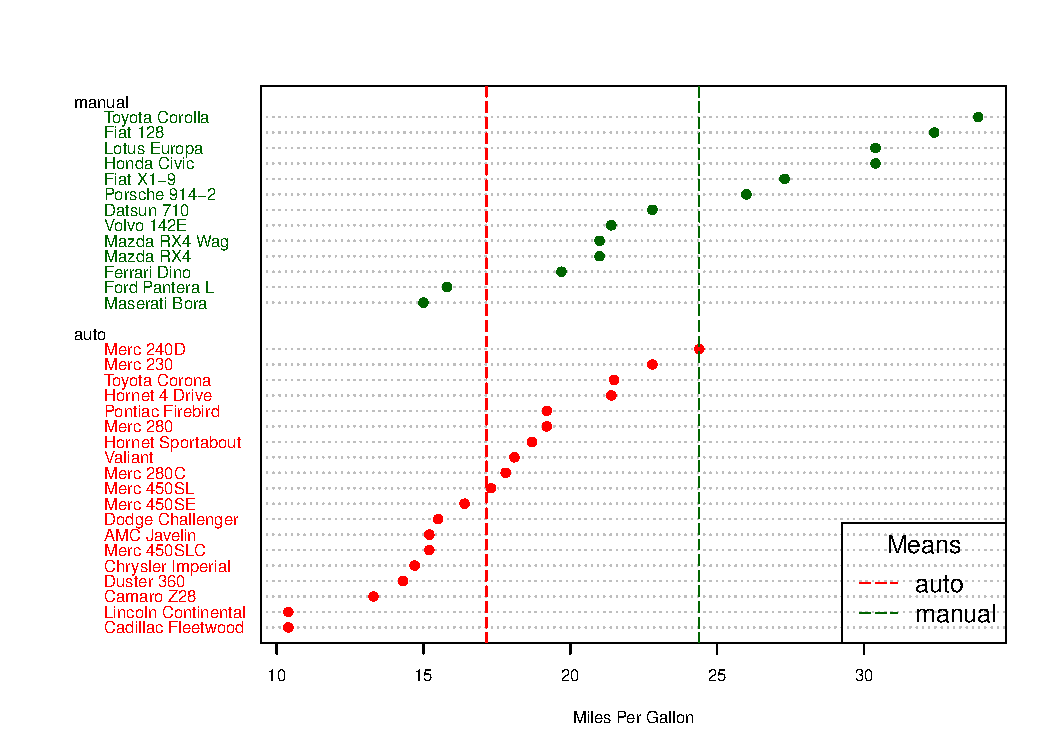
\includegraphics[width=\maxwidth]{figure/MPGTrans-1} 

}

\caption[Gas mileage grouped by transmission type]{Gas mileage grouped by transmission type}\label{fig:MPGTrans}
\end{figure}


\end{knitrout}

\begin{knitrout}
\definecolor{shadecolor}{rgb}{0.969, 0.969, 0.969}\color{fgcolor}\begin{figure}
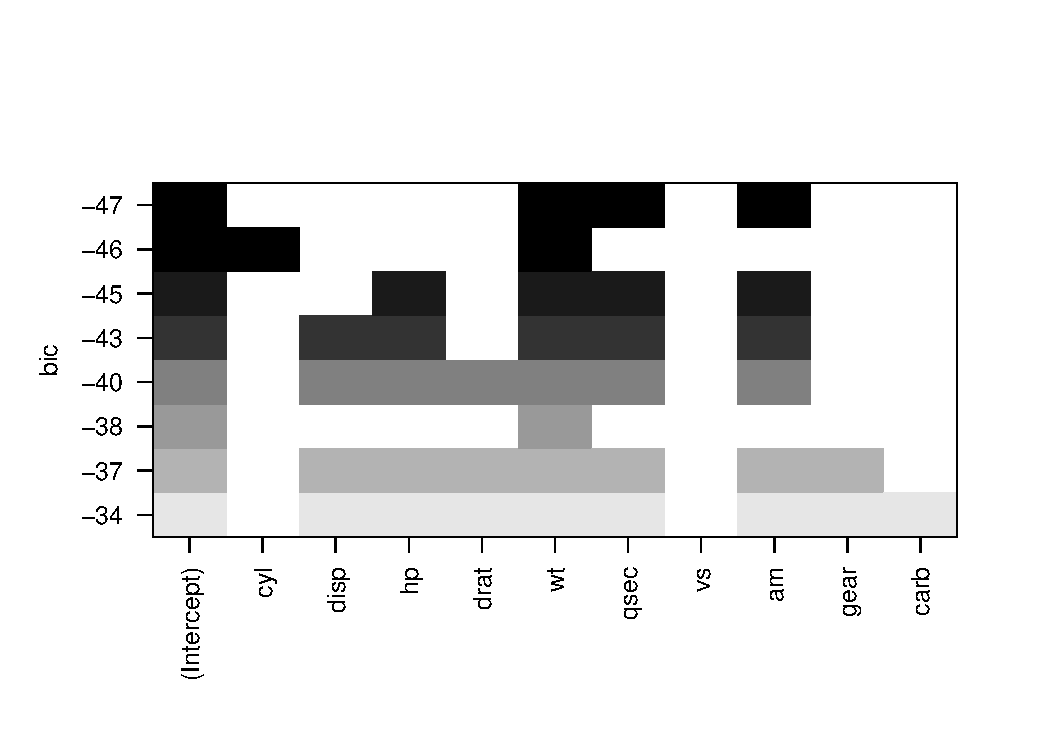
\includegraphics[width=\maxwidth]{figure/leaps-1} \caption[Determination of the best predictors]{Determination of the best predictors}\label{fig:leaps}
\end{figure}


\end{knitrout}
\begin{knitrout}
\definecolor{shadecolor}{rgb}{0.969, 0.969, 0.969}\color{fgcolor}\begin{figure}[!h]
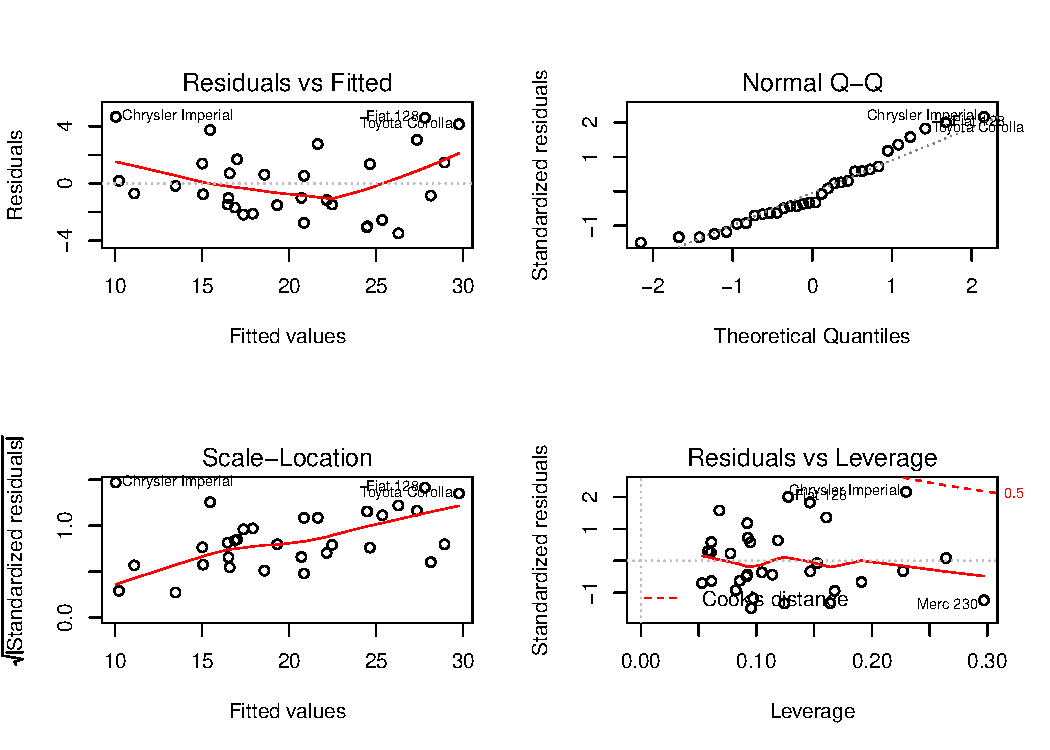
\includegraphics[width=\maxwidth]{figure/verif-1} \caption[Diagnostic plots for the regression of mpg]{Diagnostic plots for the regression of mpg}\label{fig:verif}
\end{figure}


\end{knitrout}

\begin{knitrout}
\definecolor{shadecolor}{rgb}{0.969, 0.969, 0.969}\color{fgcolor}\begin{figure}
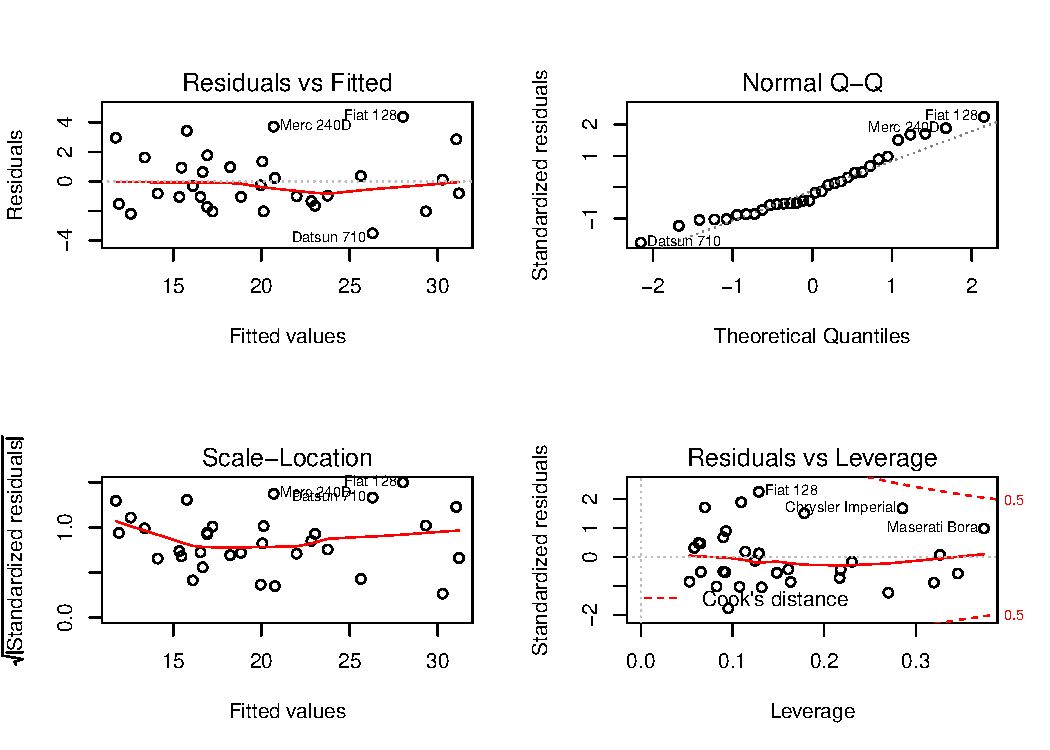
\includegraphics[width=\maxwidth]{figure/noInter-1} \caption[Improved fit model]{Improved fit model}\label{fig:noInter}
\end{figure}


\end{knitrout}
\end{document}
